% !TeX root = ../main-paper.tex

\section{A two-stage pipeline to assess OCR and NER performances on historical texts}
\label{sec:pipeline-summary}

\begin{figure}[h!]
    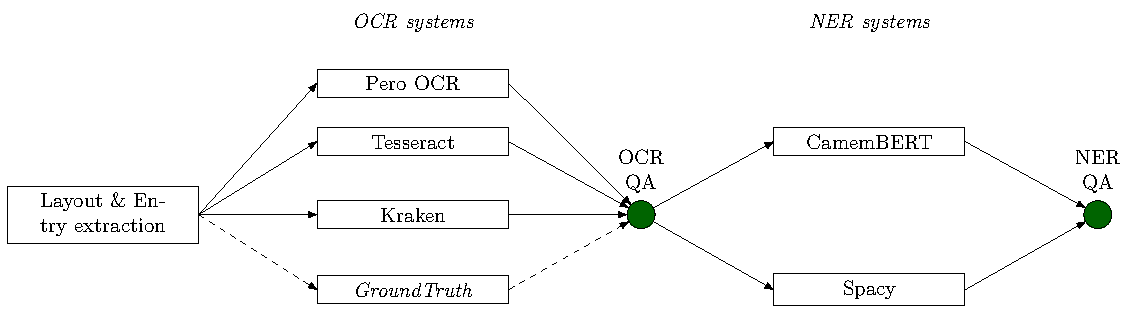
\includegraphics[width=\linewidth]{figs/protocol.pdf}
    \caption{Data extraction pipeline with two quality control checkpoints. The
    NER Q.A. checkpoint may either assess the NER system lonely (the dashed
    \emph{groundtruth} path) or may evaluate the joint work of a NER
    system with an OCR system.}
    \label{fig.pipeline}
\end{figure}


The proposed pipeline to evaluate the extraction and annotation of historical directories is depicted in~\cref{fig.pipeline}
First, the page layout extraction and entry segmentation are performed with a
semi-automated system and checked by a human.
The resulting images are the inputs of a customizable two-stage pipeline detailed in this section.


\subsection{OCR and NER systems considered}
\label{subsec:ocr-ner-tools}
We chose to test three OCR systems: Tesseract, \peroocr, and Kraken. 
We also adopt two deep-learning-based French language models, available in packaged software libraries, already trained for the NER task and that we can adapt to the domain of historical directories: SpaCy NLP pipelines and CamemBERT.
In \cref{sec:dataset}, we will explain the evaluation protocol used to assess the combined performance of these OCR and NER systems. 

\textbf{Tesseract} is a long-living project, born as a closed-sourced OCR at Hewlett-Packard in the eighties, it was progressively modernized, then open-sourced in 2005. From 2006 until November 2018, it was developed by Google and is still very active. We used in our tests version 4.1.1, released Dec. 26, 2019. Version 5, released on Nov. 30, 2021, has not been integrated in our tests yet.

\textbf{Kraken} is a project created by Benjamin Kiessling several years ago (development can be traced back to 2015), and is actively used in the open-source eScriptorium project \cite{kiessling_escriptorium_2019}.
As no pre-trained model for modern French was easily available, we used the default English text recognition model trained on modern printed English by Benjamin Kiessling on 2019. Models can be easily found and downloaded thanks to their hosting on Zenodo.

\textbf{\peroocr} is a very recent project (started in 2020) from the Brno University of Technology in Czech Republic.
Their authors used many state-of-the-art techniques to train it very efficiently.
We used the version from the master branch of their GitHub repository, updated on Sep 15, 2021.
We used the pre-trained weights provided by the authors on the same repository, created on Oct. 9, 2020 from European texts with Latin, Greek, and Cyrillic scripts.
% https://github.com/DCGM/pero-ocr
% https://www.fit.vut.cz/~ihradis/pero/pero_eu_cz_print_newspapers_2020-10-09.tar.gz

\textbf{SpaCy} is a software library that offers NLP components assembled in modular pipelines specialised by language.
Although BERT is available in the latest version of SpaCy (v3), the pipeline for French does not provide a NER layer at the time of our experiments (as of January 2022).
Hence, we rely on SpaCy's ad hoc pipeline trained on French corpora and capable of Named Entity Recognition.
% deep-sequoia and wikiner-fr, capable of named entity recognition.\textit{fr\_core\_news\_lg}\footnote{https://spacy.io/models/fr} trained two corpora in French: deep-sequoia and wikiner-fr, capable of named entity recognition.
The global architecture of these pipelines have not been yet published but are explained by the developers on their website.
Words are first encoded into local context-aware embeddings using a window-based CNN similar to~\cite{collobert2011}.
The decision layer is an adaptation of the transition-based model presented in~\cite{lample2016}.
As words are processed sequentially, their vectors are concatenated with those of the last known entities to encode the nearby predicted semantics.
The classification layer relies on a finite-state machine whose transition probabilities are learnt using a multi-layer perceptron.
% \bertrand{Drop the next sentences if we need space}
% In 2018~\cite{won2018} evaluated SpaCy's NER ability to detect place names in five corpora of ancient letters written in English.
% They measured an average F1 score of 0.57.
% The SpaCy developers claim an accuracy of 0.85 for the English NER pipeline \textit{en\_core\_web\_lg} on the OntoNotes 5.0 corpus\footnote{https://spacy.io/usage/facts-figures}.
%For our experiments, the French model \textit{fr\_core\_news\_lg} is fine-tuned using our ground truth corpus.


\textbf{CamemBERT} is well-known adaptation of the BERT transformer-based model for the French language\cite{vaswani2017attention,devlin2018bert,martin-etal-2020-camembert}. Such language models have become a new paradigm for NER\cite{li2020}. 
The learned embeddings can be used as distributed representations for input instead of traditional embeddings like Google Word2Vec, and they can be further fine-tuned for NER by adding an additional output layer, usually referred as a "head". 
They can also be pre-trained in an unsupervised way on large amount of unlabeled texts for domain adaptation.



\subsection{Metrics for OCR and NER Quality Assessment}

\begin{figure}[tb]
    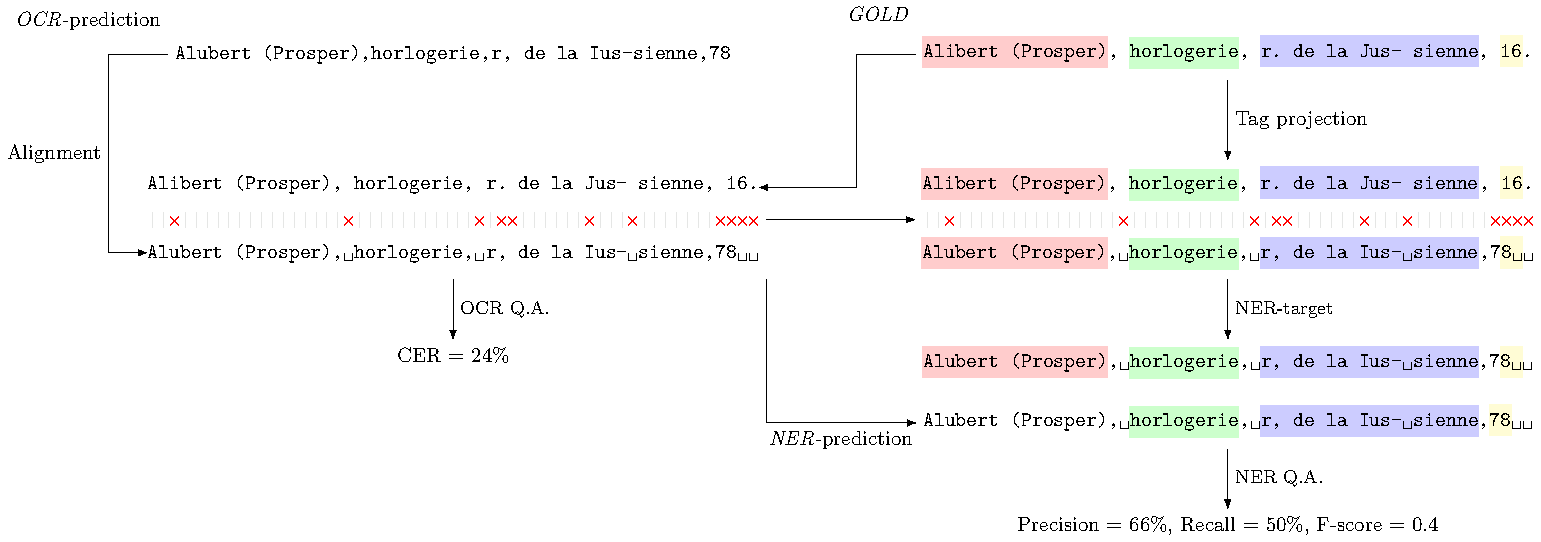
\includegraphics[width=\linewidth]{figs/eval-ocr-ner.pdf}
    \caption{OCR and NER evaluation protocol example.}
    \label{fig.eval-ocr-ner}
\end{figure}

\textbf{OCR Q.A.}  The predicted text by the OCR system is aligned with the groundtruth text using standard tools from
Stephen V. Rice's thesis~\cite{santos.2019.wcmel,neudecker.2021.whdip}. The Character Error Rate (CER) is computed at
the entry level and at the global level, defined as the ratio between the number of errors
(insertions/deletions/substitutions) over the reference text length.
Word Error Rate is hard to define for our tokens and was not considered.

%In this benchmark, we consider 3 OCR systems well known for historical document analysis: Pero OCR, Tesseract, and Kraken. 


\textbf{NER Q.A.}. The NER system outputs a text with tags that enclose the entities. To assess the quality of the
entity extraction, we rely on a technique similar as for the OCR evaluation to build the \emph{NER-target}. The
\emph{NER-target} is different from the groundtruth because it should not involve the errors committed during the
previous stages. The OCR text is first aligned with the groundtruth text to form the NER-\emph{input} (where
\emph{input} is a placeholder for \emph{pero} if the input text is from PERO, NER-\emph{tesseract},
NER-\emph{reference}\ldots). The tags of the groundtruth are then projected in the alignment on NER-\emph{input} to
provide the \emph{NER-target}. The NER system then runs on NER-\emph{input} and outputs the \emph{NER-prediction}. The
precision, recall, and f-measure (or f-score) are computed considering only the exact matches between entities of the
\emph{NER-target} and those from the \emph{NER-prediction}, i.e. pairs of entries for which the type, start and end positions are exactly the same.
Precision is the ratio of exact matches divided by the number of predicted entries,
and recall is defined as the ratio of exact matches divided by the number of expected entries;
the f-measure is their harmonic mean.

The evaluation process is illustrated on~\cref{fig.eval-ocr-ner}. The OCR and the groundtruth texts are first aligned to
evaluate the OCR accuracy. As there are 11 mismatches over 56 aligned characters, the CER is thus 24\%. This alignment
is then used to back-project the groundtruth tags to build the tagged NER-\emph{target}. Finally, the NER system runs on the
OCR text; its output is compared to the NER groundtruth. There is only 2 over 3 tags matching in the prediction (precision),
while only 2 over 4 entities are matched in the reference (recall). It follows an overall f-score of 0.4.
%
% A side effect of tag projection is that it can produce degenerated tags, i.e. empty or containing only spaces.
% In such cases, the corresponding entries must be removed from the dataset,
% and only the intersection of the sets of valid entries must be used to compare NER systems with multiple OCR predictions or references.
